\documentclass[11pt]{article}
\usepackage[utf8]{inputenc}
\usepackage[T1]{fontenc}
\usepackage[margin=2.4cm]{geometry}
\usepackage{amsmath,amssymb}
\usepackage{graphicx}
\usepackage{subcaption}
\usepackage{booktabs}
\usepackage{tikz}
\usetikzlibrary{arrows.meta,positioning}
\usepackage[hidelinks]{hyperref}
\usepackage{caption}
\captionsetup{font=small,labelfont=bf}
\usepackage[section]{placeins}

% Let large figures actually sit on text pages instead of drifting to the end.
\renewcommand{\topfraction}{0.9}
\renewcommand{\bottomfraction}{0.6}
\renewcommand{\textfraction}{0.07}
\renewcommand{\floatpagefraction}{0.75}

% Figures: keyboard frames live in ../assets, exported result frames in figures/
% (regenerate with src/export_report_figures.m)
\graphicspath{{figures/}{../assets/}}

% --- Local-build fallback: missing figures render as a placeholder box instead
% of aborting compilation. Existing images (found in . / figures/ / ../assets/)
% are shown normally, so this is harmless on Overleaf and for teammates.
\makeatletter
\let\orig@includegraphics\includegraphics
\renewcommand{\includegraphics}[2][]{%
  \IfFileExists{#2}{\orig@includegraphics[#1]{#2}}{%
   \IfFileExists{figures/#2}{\orig@includegraphics[#1]{#2}}{%
    \IfFileExists{../assets/#2}{\orig@includegraphics[#1]{#2}}{%
     \fbox{\parbox[c][0.22\textwidth][c]{0.9\linewidth}{\centering\ttfamily [figura mancante: \detokenize{#2}]}}}}}}
\makeatother

% =====================================================================
% TITLE BLOCK
% =====================================================================
\title{\textbf{Visual reconstruction of played notes on a piano keyboard\\
from a single top-view video}}
\author{
  Flavio De Lellis \and
  Filippo Garofalo \and
  Emanuele Turbanti \\[4pt]
  \small Image Analysis and Computer Vision, Politecnico di Milano
}
\date{\today} % TODO set the delivery date

\begin{document}
\maketitle

\begin{abstract}
\noindent
We present a pipeline that takes an ordinary RGB video of two hands playing a
piano, filmed roughly from above, and marks on every frame which keys are being
pressed. The system uses only classical image processing and projective
geometry, with no learning involved and a single short manual calibration. Our
contribution over similar course projects is twofold. First, the keyboard is
rectified through a homography that we estimate from scratch with a normalized
Direct Linear Transform, and the key grid is then built analytically in
millimetres so that both white \emph{and} black keys are modelled. Second, the
press decision combines a spatial cue (a finger lies on the key) with a temporal
cue (the key surface actually changed), where the temporal stage uses a
two-channel frame difference, darkening for white keys and signal magnitude for
black, measured only on each key's exposed surface. A key
is reported as pressed only when both cues agree. We tested the method on five
videos with very different lighting, backgrounds and hand styles.
\end{abstract}

\section{Introduction}
The goal of this project is simple to state and surprisingly hard to do well:
given a video of someone playing the piano, recover which notes are sounding at
each instant, using nothing but the picture. We deliberately stay with a
single, fixed, roughly top-down camera, because that is the cheapest setup a
student or a hobbyist already owns. The output is the original video with the
pressed keys painted on top, keeping the link between each pressed key and the
finger responsible for it visible.

The motivation comes mostly from Music Information Retrieval, where automatic
transcription tries to turn a performance into a symbolic score or a MIDI
file~\cite{benetos2019transcription}. Audio based transcription is the usual
route, but it has well known trouble with dense polyphony, with notes that
overlap and with instruments that are slightly out of tune. Looking at the
player's hands sidesteps part of that, because the physical contact between a
finger and a key is unambiguous in a way that mixed audio is not. The same idea
has obvious uses in tutoring: a system that can see a wrong finger or a wrong
timing could give feedback to a student practising at home, which matters for
remote teaching.

There is also a plain computer vision reason to care. Hands on a piano are about
the worst case for hand tracking. They are not posed to help the camera, they
occlude each other constantly, fingers curl down toward the keys so the
fingertips disappear, and a finger can rest on a key without playing it. A
method that copes with this is a method that copes with a lot.

\section{Method}

\subsection{Overview}
We stay deliberately on the cheap end of the hardware spectrum: a single RGB
camera, no depth sensor and no second viewpoint, and no learned component
anywhere in the chain. Adding hardware would make the problem easier (a frontal
camera or a depth sensor measures key travel directly~\cite{akbari2015pianodepth},
and a CNN could absorb much of the appearance variation), but each of those
options carries a cost, in equipment or in annotated data, that a setup meant to
run on footage anyone can shoot should not assume. Working inside that
constraint is the whole point, and Figure~\ref{fig:pipeline} shows how we do it.

The pipeline has a one-time calibration and then a per-frame loop. Calibration
recovers the geometry of the keyboard and freezes a virtual key grid. The loop
runs two parallel branches on every frame: a \emph{spatial} branch that asks
which keys have a fingertip over them, and a \emph{temporal} branch that asks
which keys have visually changed with respect to a resting reference. A key is
declared pressed only when it appears in both branches at once. Figure~\ref{fig:pipeline}
sketches the flow.

\begin{center}
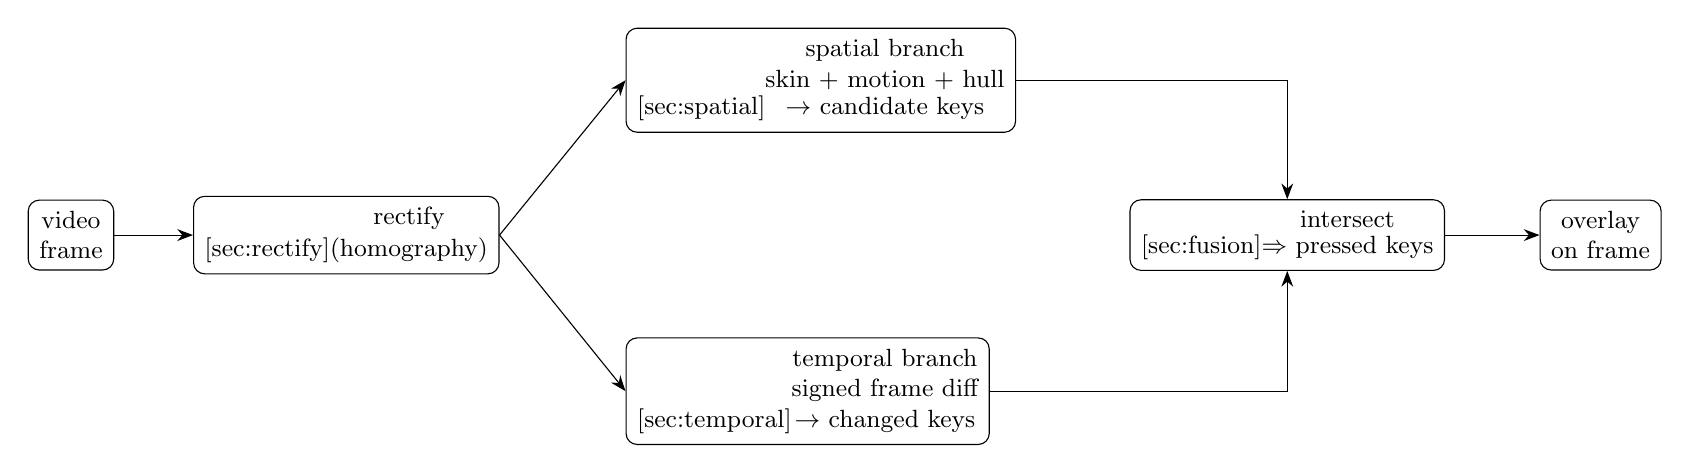
\begin{tikzpicture}[
  node distance=6mm and 9mm,
  box/.style={draw, rounded corners, align=center, font=\small, inner sep=4pt, minimum height=8mm},
  >={Stealth[length=2mm]}
]
\node[box] (frame) {video\\frame};
\node[box, right=10mm of frame] (rect) {\hyperref[sec:rectify]{\shortstack{rectify\\(homography)}}};
\node[box, above right=8mm and 16mm of rect] (spatial) {\hyperref[sec:spatial]{\shortstack{spatial branch\\skin + motion + hull\\$\rightarrow$ candidate keys}}};
\node[box, below right=8mm and 16mm of rect] (temporal) {\hyperref[sec:temporal]{\shortstack{temporal branch\\signed frame diff\\$\rightarrow$ changed keys}}};
\node[box, right=80mm of rect] (fuse) {\hyperref[sec:fusion]{\shortstack{intersect\\$\Rightarrow$ pressed keys}}};
\node[box, right=12mm of fuse] (out) {overlay\\on frame};
\draw[->] (frame) -- (rect);
\draw[->] (rect.east) -- (spatial.west);
\draw[->] (rect.east) -- (temporal.west);
\draw[->] (spatial.east) -| (fuse.north);
\draw[->] (temporal.east) -| (fuse.south);
\draw[->] (fuse) -- (out);
\end{tikzpicture}
\captionof{figure}{High level structure. Calibration (not shown) runs once and
produces the homography and the virtual key grid that both branches rely on.}
\label{fig:pipeline}
\end{center}

\subsection{Geometric calibration and rectification}
\label{sec:rectify}
Because the camera sits at a slight angle to the keyboard normal, the keys appear
as a trapezoid rather than a rectangle, and reasoning about key positions
directly in pixels is fragile. We remove this distortion with a planar
homography. The top faces of the white keys lie on a single plane $\pi$, and the
image of that plane is related to the plane itself by
\begin{equation}
  \mathbf{u} \sim \mathtt{H}\,\mathbf{x}, \qquad
  \mathbf{u}=[x,y,1]^{\top}, \quad \mathbf{x}=[X,Y,1]^{\top},
\end{equation}
where $\mathbf{x}$ is a point on the keyboard plane in millimetres and
$\mathbf{u}$ is its pixel in the frame. We do not call a library routine for
this. The operator clicks the four corners of the visible white-key region once,
those corners are ordered as top-left, top-right, bottom-right, bottom-left from
the signs of their coordinate sums and differences, and they are matched to a
metric rectangle whose width is (number of white keys) $\times 23.5$ mm and whose
height is $150$ mm.

The homography is then estimated with a Direct Linear
Transform~\cite{hartley2004multiple}. Each correspondence contributes two rows to
a $2n \times 9$ matrix $\mathtt{A}$,

and the solution is the right singular vector of $\mathtt{A}$ associated with the
smallest singular value, reshaped into the $3\times 3$ matrix $\mathtt{H}$ and
scaled so that $H_{33}=1$. We keep both $\mathtt{H}$ and its inverse, since the
two branches need opposite directions: rectifying an image needs plane to image,
while mapping a detected fingertip back onto the keyboard needs image to plane.


Rectification itself is done by inverse warping. We build the output grid in the
metric plane at a chosen resolution (we used $4$ pixels per millimetre), send
each output pixel through $\mathtt{H}$ into the source frame, and sample there
with bilinear interpolation. The result is a clean top-down image of the keys on
which every later step operates. The four corners double as a region of interest
mask: anything outside the clicked quadrilateral, in particular the red felt
strip above the keys that otherwise pollutes skin detection, is discarded before
segmentation. Figure~\ref{fig:rectify} shows the result on one of our frames.

\begin{figure}[!htb]
\centering
\begin{subfigure}[t]{0.46\textwidth}
  \centering
  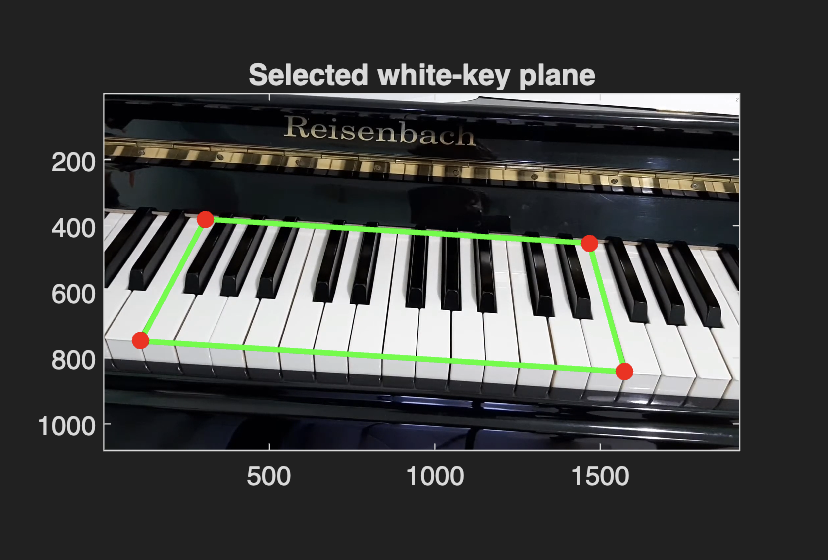
\includegraphics[width=\textwidth]{calib_corners.png}
  \caption{Source frame with the four clicked corners (red) and the resulting
  white-key quadrilateral (green), which also serves as the region of interest.}
  \label{fig:rectify-corners}
\end{subfigure}\hfill
\begin{subfigure}[t]{0.52\textwidth}
  \centering
  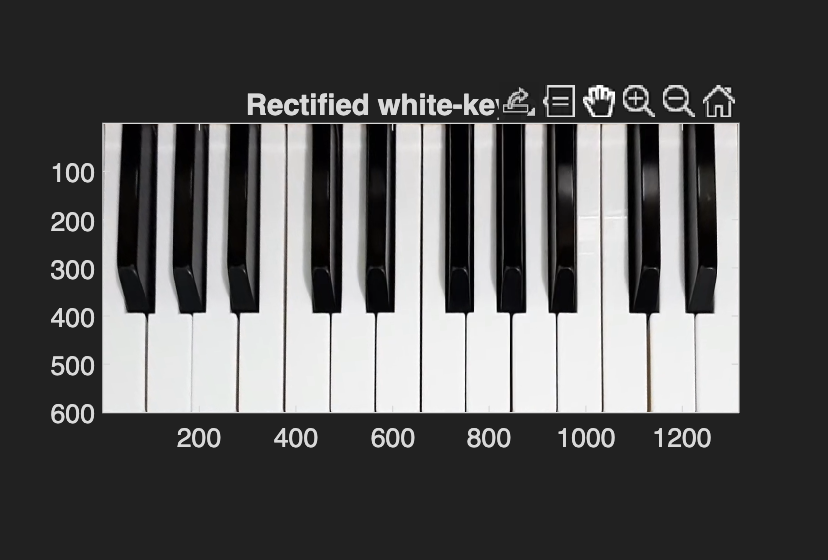
\includegraphics[width=\textwidth]{calib_rectified.png}
  \caption{The same region after inverse warping with $\mathtt{H}$: a metric,
  top-down view of the keys at $4$ pixels per millimetre.}
  \label{fig:rectify-rect}
\end{subfigure}
\caption{Calibration and rectification on a frame of one test video ($14$ white
keys, leftmost note C). The homography straightens the slanted keyboard into the
rectangular plane on which every later stage operates.}
\label{fig:rectify}
\end{figure}

\FloatBarrier
\subsection{The virtual keyboard model}
Once the plane is metric we never measure key positions from the image again. We
generate them. White keys are an even partition of the calibrated width into
equal columns. Black keys are placed analytically from the standard octave
pattern $[1\,1\,0\,1\,1\,1\,0]$ (reading the white notes C,D,E,F,G,A,B, a $1$
meaning a black key sits to the right of that white). The pattern is rotated to
start on the leftmost visible note, which the user supplies, and tiled across the
visible range.

The constants
($w_w=23.5$ mm, $w_b=13.7$ mm, white length $150$ mm, black length $95$ mm) live
in a single file, so changing the geometry propagates everywhere with no manual
retuning. The end product is one array of keys, each carrying its polygon both
in millimetres and in rectified pixels, its bounding box and its type. This is
the shared map that the spatial and temporal branches both query. Handling black
keys at all is something the reference projects we looked at left as future work,
and the analytic placement is what made it tractable for us.
Figure~\ref{fig:vkgrid} overlays the generated grid on the rectified plane.

\begin{figure}[!htb]
\centering
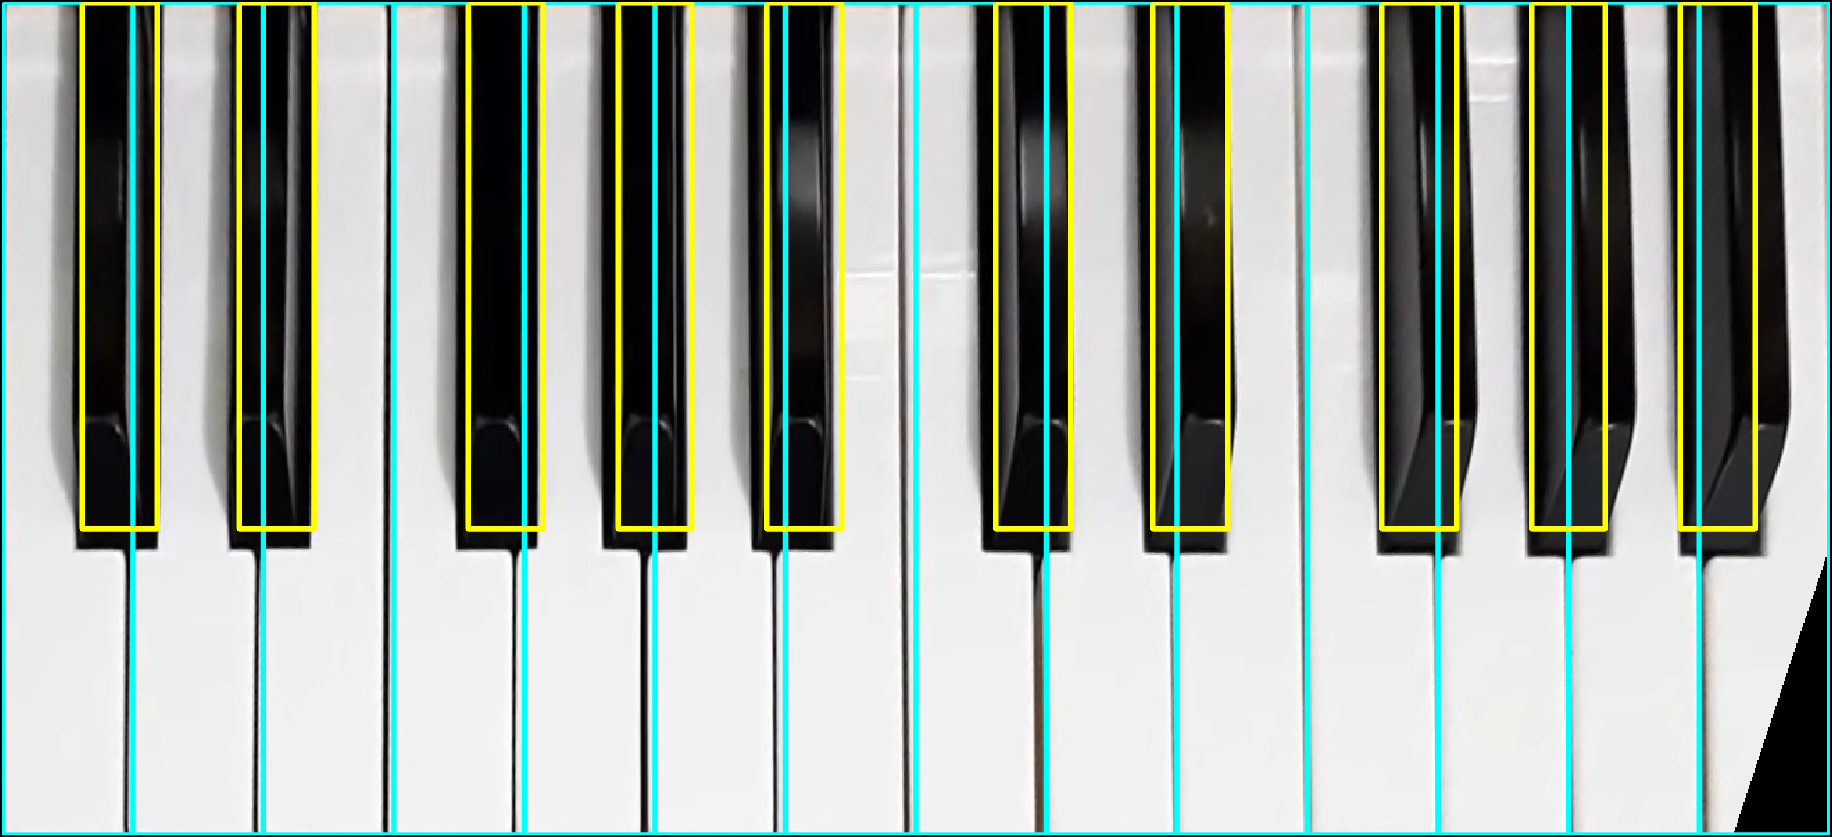
\includegraphics[width=0.82\textwidth]{calib_grid.png}
\caption{The virtual keyboard model drawn over the rectified plane}
\label{fig:vkgrid}
\end{figure}

\FloatBarrier
\subsection{Spatial branch: from pixels to candidate keys}
\label{sec:spatial}
The spatial branch answers a narrow question, which keys have a finger over them,
and it is allowed to over-answer, since the temporal branch will prune it.

\paragraph{Skin and motion.}
Skin is segmented in YCbCr, which separates luminance from chrominance and is a
common choice for this exact task~\cite{benabdelkader2005ycbcr}. We keep pixels
with $Y\in[100,235]$, $C_b\in[85,135]$, $C_r\in[135,180]$. On its own this also
fires on ivory keys, whose colour is close to pale skin, so we add a simple but
effective constraint: hands move and keys do not. We build a motion mask by thresholding 
the absolute grayscale difference between the current frame and the resting reference 
(using a threshold of $40$ out of $255$). Intersecting the skin mask with this motion 
mask removes the static ivory blobs that would otherwise turn into phantom fingers. 
Finally, we clean the mask with standard morphological operations, closing it with a 
$5$-pixel disk to bridge gaps, filling internal holes, and dropping any isolated 
components smaller than $50$ pixels.

\paragraph{Separating the two hands.}
We apply connected component labeling to isolate independent blobs. We keep at most 
the two largest components, provided their area $A_i$ satisfies an adaptive floor:
\begin{equation}
    A_i \geq \max\left(1000,\, 0.4 \times \max_j A_j\right)
\end{equation}
The relative term is what lets a real second hand through while still rejecting a 
distant reflection or shadow: a true second hand has an area comparable to the 
dominant component, whereas a reflection does not.

\paragraph{Fingertips by convex hull.}
Because a hand is a highly non-convex shape with deep valleys between the fingers, 
its raw contour is complex to track. To find the fingertips, we instead compute the 
convex hull of each hand blob. Intuitively, the convex hull is the shape a rubber 
band would take if stretched around the entire hand; the points where the band is 
forced to bend sharply are the protruding fingertips. 

We compute this using a custom implementation of the Graham scan~\cite{graham1972convexhull}. 
The algorithm begins by finding an anchor point guaranteed to be on the outer boundary: 
the pixel with the lowest $y$-coordinate (the base of the hand in the image), breaking 
ties with the smallest $x$-coordinate to yield $p_0 = (x_0, y_0)$. We then imagine a ray 
sweeping counter-clockwise from this anchor and sort every other pixel $p_i = (x_i, y_i)$ 
by its polar angle $\theta_i = \text{atan2}(y_i - y_0, x_i - x_0)$.

With the points sorted, we build the hull perimeter by pushing points onto a stack. 
To ensure the boundary always remains convex, we test the last three points: $p_1$ 
(second to top of stack), $p_2$ (top of stack), and $p_3$ (the new candidate). 
We calculate the 2D cross product of the vectors forming this turn:
\begin{equation}
    CP = (x_2 - x_1)(y_3 - y_1) - (y_2 - y_1)(x_3 - x_1)
\end{equation}
If $CP > 0$, the path makes a valid left turn, and $p_3$ is pushed onto the stack. 
If $CP \le 0$, the path makes a right turn, meaning $p_2$ forms a concavity (such as 
the webbing between two fingers). We pop $p_2$ off the stack, pulling the boundary 
tight over the gap, and repeat the test.

The resulting hull gives us the outer boundary points of the hand, but this includes 
the sides of the palm and the wrist. We isolate the functional fingertips using three 
spatial heuristics. First, we calculate the robust median $y$-coordinate of the hand 
blob and instantly discard any hull vertex falling below this horizontal bisector. 
Second, because a single rounded fingertip might trigger a cluster of adjacent vertices, 
we merge any candidates closer than $35$ pixels. Crucially, during this merge, we 
retain the coordinates of the candidate with the minimum $y$-value, ensuring the logged 
point correctly represents the absolute physical apex of the finger. Finally, we discard 
any vertex within $20$ pixels of the frame border, as hands cut off by the camera's 
field of view produce artificial hull corners. 

\paragraph{Mapping fingertips to keys.}
Each fingertip, detected in the original frame as homogeneous coordinates $\mathbf{u} = [x, y, 1]^\top$, 
is mapped to the rectified metric plane $\mathbf{x}_{rect}$ via the inverse homography matrix:
\begin{equation}
    \mathbf{x}_{rect} \sim \mathtt{H}^{-1} \mathbf{u}
\end{equation}
We then test black keys before white ones, because a black key physically sits on top 
of the rear portion of the whites. The test is not exact, though, and the reason is 
parallax. The homography is calibrated on the plane of the white keys. However, black 
keys and knuckles lie at an elevation above that plane, causing their projection to 
shift artificially forward in the image. We compensate for this with vertical 
tolerances tuned on the videos: $80$ pixels of slack when testing black-key boxes 
and $60$ pixels when testing white-key polygons. A fingertip matches the first black 
box that contains it (within tolerance); otherwise, it is shifted back and tested 
against the white polygons.

\paragraph{Candidate expansion across a chord.}
A finger rarely sits dead centre on a key, and a hand spanning a chord often
triggers only some of the keys it actually covers. When two or more candidates
are present, we sort them horizontally. We split them into separate groups wherever 
the spatial gap between consecutive candidates exceeds three white-key widths, 
which effectively detects the empty space between the left and right hands. 
Each group is then filled in to span its full horizontal extent. In this way, a hand 
resting across several keys reports all of them as spatial candidates, while the 
empty gap between the two hands is logically preserved.

\subsection{Temporal branch: did the surface actually change?}
\label{sec:temporal}
The spatial branch cannot tell a pressed key from a key merely touched, because
from above they look almost identical. The temporal branch resolves this by
comparing each frame against a resting reference, which we take to be the first
rectified frame. This reference must be a clean frame: the keyboard at rest and
\emph{no hands on it}. Since every later frame is judged against it, a hand or an
already-pressed key present in the reference would corrupt the baseline and leak
into the difference as a spurious change. We therefore require the video to begin
on such a frame, before the player's hands enter the keyboard.

From a grayscale difference $g = \text{gray}(\text{current}) -
\text{gray}(\text{reference})$ we build two complementary channels, one per key
type, because white and black keys change in opposite ways. A white key is light
(ivory), and a press darkens its surface: both the finger and the contact shadow
it casts are darker than the key, so on a white key a press appears as a drop in
brightness ($g<0$). The white channel therefore keeps only the darkened pixels and
discards any brightening, which on a white key is almost always spurious. A black
key is the opposite case: it is dark and narrow, so its press signal is weak and
goes \emph{both} ways --- the contact shadow darkens its edges, while skin and
reflections at the borders can lighten it. Keeping the brightening alone lost most
black presses, so the black channel takes the full \emph{magnitude} of $g$:
\begin{equation}
  d_{\text{white}} = \frac{\max(0,-g)}{255}, \qquad
  d_{\text{black}} = \frac{|g|}{255}.
\end{equation}
Figure~\ref{fig:temporal} shows the difference and the two channels on a frame
with a black key down.

A finger over a key is not, by itself, a press: it may merely rest on it or pass
above it. What marks a real press is that the \emph{exposed} surface of the key
changes, through the contact shadow and the slight displacement of the key. We
therefore remove the skin (the hand mask, warped into the rectified plane) from
\emph{both} channels, so each key is judged only on the part of its surface the
finger does not cover, never on the finger itself.

Each channel is then binarized against a per-type threshold --- a tunable
parameter, set to $30/255$ in most of our runs --- and the resulting binary mask is
cleaned of isolated noise pixels.
Then, for every key, we restrict the analysis to the adaptive band described below,
shrink the region by a two-pixel inner margin to reduce bleed from neighbours, 
and compute the fraction of changed pixels \emph{over the exposed area} of the key,
\begin{equation}
  r_k = \frac{\text{changed, non-skin pixels}}{\text{non-skin (exposed) pixels}},
\end{equation}
declaring the key changed when $r_k$ passes a per-type level ($10\%$ for white,
$20\%$ for black). Normalising over the exposed area, rather than the whole
region, is what lets us strip the skin without diluting the score: on a narrow
black key the finger covers most of the surface, and dividing by the full region
would drag every ratio below threshold. A guard abstains when too few exposed
pixels remain. The analysis band is the key safeguard here: rather than a fixed
top third as in previous solutions, it tracks the highest detected fingertip frame
by frame and cuts just above it (with a floor of $15\%$ of the keyboard height),
so the fingers and --- under proper frontal lighting, where they fall below the 
contact point --- their cast shadows are left out of the per-key statistics entirely.

\begin{figure}[!t]
\centering
\begin{subfigure}{\textwidth}
  \centering
  \includegraphics[width=0.8\textwidth]{temporal_diff.png}
  \caption{Signed difference against the reference frame: blue where the surface
  got darker, red where it got lighter. The pressed black key shows up as the
  strong red column on the right; most of the blue is the hand, which the skin
  mask removes from both channels before the per-key counting.}
  \label{fig:temporal-diff}
\end{subfigure}

\vspace{5pt}
\begin{subfigure}{\textwidth}
  \centering
  \includegraphics[width=0.8\textwidth]{temporal_channels.png}
  \caption{The two thresholded channels over the key grid, white channel in
  green and black channel in red. The cyan line is the adaptive cut just above
  the highest fingertip: only pixels above it are counted, so the hand and arm
  below stay out of the per-key statistics.}
  \label{fig:temporal-channels}
\end{subfigure}
\caption{The temporal branch on the same frame as Figure~\ref{fig:result}.}
\label{fig:temporal}
\end{figure}

\subsection{Fusion}
\label{sec:fusion}
The two branches each return a set of key indices. The reported pressed keys are
their intersection: a key must have a fingertip over it \emph{and} have changed
with respect to rest. This single AND is what removes the bulk of the false
positives, since a hovering hand satisfies the spatial test but not the temporal
one, and a shadow or reflection satisfies neither cleanly. The final overlay
marks the projected fingertips and fills the confirmed presses, green on white
keys and red on black ones, on top of the rectified frame.

\section{Experiments and results}
\label{sec:results}
We recorded and collected five videos to stress different parts of the pipeline:
four from public online sources and one filmed by us in a normal room. They vary
in lighting, in background clutter, in whether the instrument is an acoustic
grand or an electronic keyboard, and in hand morphology and posture. All of them
start on a resting frame, which the temporal stage needs as its reference. Three
are representative enough to describe here, and Figure~\ref{fig:result} shows the
final output on two frames of one of them.

\begin{figure}[!t]
\centering
\begin{subfigure}{0.49\textwidth}
  \centering
  \includegraphics[width=\textwidth]{result1.png}
  \caption{}
  \label{fig:result-a}
\end{subfigure}\hfill
\begin{subfigure}{0.49\textwidth}
  \centering
  \includegraphics[width=\textwidth]{result2.png}
  \caption{}
  \label{fig:result-b}
\end{subfigure}
\caption{Final output on two processed frames. Confirmed presses are filled,
green on white keys and red on black ones; the red stars are the fingertips
after projection onto the rectified plane. The fill follows the visible key
surface rather than the bounding box, so it stops at the finger and at the
neighbouring keys.}
\label{fig:result}
\end{figure}

The first video shows a baby grand under good, high-contrast light, but the
camera is clearly off the keyboard normal, so the projective distortion is large.
This makes it a good test of the calibration: once rectified, the keys line up
with the virtual grid and the rest of the pipeline behaves as if the camera had
been overhead. The pianist plays with a pronounced claw posture, so several
fingertips are hidden and the convex hull misses them. Because a press needs both
cues, a key whose fingertip is missed is not reported, even when its surface has
clearly changed: this posture is exactly where the spatial branch limits recall.
Where a fingertip is still detected, the press is confirmed cleanly, since the
temporal change on that key is unambiguous.

The second video is an electronic keyboard against a busy, multicoloured
background, with shadows between the black keys. The camera here is close to an
ideal top-down view. This case mostly tests robustness of skin segmentation to
background clutter; the motion gate is what carries it, since the colourful
background is static and never enters the skin-and-motion intersection.

The third video is the one we filmed at home, and it is the hardest. Both hands
play at once, the light is poor, and the wood of the instrument is close in colour
to the skin, so chromatic contrast is low. This is the only case where we had to
nudge the skin thresholds by hand. With that adjustment the system still
separates the two hands correctly through the connected-component step and reports
plausible presses on both.

Across the set, the pipeline marks pressed white keys reliably under projective
distortion, cluttered backgrounds, low light and two-hand play, and it also picks
up black-key presses, which the white-only reference systems do not attempt. The
honest weak point is the candidate stage on its own: it flickers frame to frame,
and in the hardest frames it produces spurious candidates. The temporal
verification is what tames this, and the gap between the raw candidate stream and
the final, intersected output is the clearest evidence that the two-cue design
was the right call.

\section{Conclusions and open problems}
We built a single-camera, no-learning pipeline that reports pressed piano keys
from a top-view video, using a from-scratch homography for rectification, an
analytic virtual keyboard that includes black keys, a convex-hull spatial branch,
and a two-channel, exposed-surface temporal branch, fused by intersection. On a varied set
of videos it handles white and black presses under a range of real conditions.

The limitations are the ones inherent to hand-tuned classical methods. Several
thresholds (skin ranges, the motion gate, the parallax tolerances) depend on
lighting and on the instrument, and a genuinely new scene can need a touch of
retuning. A learned skin or hand model would remove much of that sensitivity, at
the price of a labelled dataset we did not have. The detection is also purely
frame-by-frame: adding tracking over time would let us reconstruct note onsets
and durations, and from there an actual transcription. Finally the field of view
covers only part of the keyboard at once, which caps the pitch range, and the
black-key cue, while working, is more delicate than the white one because of the
parallax we described in Section~\ref{sec:temporal}. These are the directions we
would take the work next.

\paragraph{Contributions.}
Flavio handled the geometric calibration, the homography and the rectification.
Filippo built the spatial branch, the skin and motion segmentation and the convex
hull. Emanuele developed the temporal branch and the press confirmation. The
fusion logic and the experiments were done jointly.

\bibliographystyle{ieeetr}
\bibliography{references}

\end{document}
